\documentclass{article}

\usepackage{RepSty}
\usepackage{SPINDefs}
\usepackage{hyperref}

\usepackage{setspace}
\usepackage{multirow}
\usepackage{threeparttable}



\begin{document}
	\singlespacing
	\begin{titlepage}

\begin{center}
{МИНИСТЕРСТВО ОБРАЗОВАНИЯ И НАУКИ РОССИЙСКОЙ ФЕДЕРАЦИИ}\\[3pt]
\textsc{\small{Федеральное государственное автономное образовательное учреждение высшего образования}}\\

\textbf{\enquote{Национальный исследовательский ядерный университет\\
{``МИФИ''}}}\\
\textbf{(НИЯУ МИФИ)}\\[2cm]




\textsc{\textbf{Отчет о научно-исследовательской деятельности\\		
		аспиранта и подготовке научно-квалификационной\\	
		работы (диссертации) на соискание ученой степени\\		
		кандидата наук за первое полугодие 2 курса}}\\[2cm]

% Title
\enquote{Исследование влияния возможных систематических ошибок на результаты эксперимента по изучению временной инваринтности на ускорителе COSY}\\[2cm]


\end{center}


\begin{flushleft}
% Author and supervisor
\begin{tabular}{ll}
Аспирант 						& А.Е. Аксентьев \\
Направление                     & 03.06.01 Физика и астрономия \\					
Научная специальность		   	& 01.04.20 Физика пучков заряженных частиц\\
								& \-\hspace{1.8cm} и ускорительная техника \\[1cm]
Научный руководитель 			& \\
Должность, степень, звание 		& С.М. Полозов, к.ф.-м.н, доц. \\[1cm]
Дата защиты:					& \\
Результат защиты:				& \\
\end{tabular}

\end{flushleft}

\vfill


\begin{center}
Москва \the\year{}
\end{center}



\end{titlepage}
	
	\tableofcontents 
	\pagebreak
	
	\onehalfspacing
	\section*{Физическая мотивация}
	Наше нынешнее понимание природы основано на Стандартной Модели (СМ) элементарных частиц. Наблюдаемая разница между предсказанным ей, и реальным, отношениями количества материи к антиматерии --- Барионная Асимметрия Вселенной (БАВ) --- фундаментальная проблема этой, в остальном чрезывчайно успешной (как подтверждается недавним открытием Бозона Хиггса на Большом Адронном Коллайдере), теории.
	
	В 1967 году, Андрей Дмитриевич Сахаров сформулировал три условия происхождения БАВ, одно из которых --- нарушение C- и CP-симметрий.~\cite{Sakharov} Фундаментальные симметрии C, P и T, в свою очередь, связаны между собой CPT-теоремой, которая подтверждена с крайне высокой точностью и считается истинной симметрией. По этой теореме, из нарушения CP-симметрии следует нарушение T-симметрии.
	
	На данный момент, практически все известные механизмы нарушения T-симметрии нарушают и P-симметрию, из-за чего нельзя утвердительно сказать нарушается ли при этом C-симметрия. До сих пор, взаимодействия нарушающие T- без нарушения P-симметрии в системе барионов не были описаны в литературе; в связи с чем, их обнаружение может свидетельствовать о физике, не описываемой СМ.
	
	Наблюдать T-нечётную, P-чётную величину --- корреляционный коэффициент реакции --- можно~\cite{Conzett} при поляризованном рассеянии протонного пучка на дейтериевой мишени. На синхротроне COSY (находящемся в исследовательском центре города Юлих, Германия) имеется уникальная возможность измерения этой величины в трансмиссионном эксперименте с использованием векторно-поляризованного протонного пучка и тензорно-поляризованной дейтериевой мишени: эксперименте TRIC (Time-Reversal Invariance at COSY).~\cite{Proposal} 
		
	\section{Состояние изучаемой проблемы}
	Эксперименты по нарушению $T$-симметрии, как правило, заключаются в измерении асимметрии реакции при обращении какой-либо величины (такой как поляризация), таким образом, чтобы получившаяся реакция была эквивалентна временному обращению изначальной.
	
	Прямым тестом нарушения $T$-симметрии в слабых взаимодействиях является эксперимент CPLEAR, в котором проводилось изучение каонных систем.~\cite{CPLEAR} Исследовалась аннигиляция $\bar{p}p \to K^+ \pi^- \bar{K}^0$ или $K^- \pi^+ K^0$. Детектируя заряженные продукты реакции, и их временную эволюцию, можно вычислить изначальную странность произведённых нейтральных каонов. После производства, каоны свободно распадались под действием слабого взаимодействия. Сравнивая количество каонов, превратившихся в антикаоны, и наоборот, можно вычислить временную асимметрию: если $T$-симметрия верна, количество превращений в одну сторону должно быть одинаково количеству превращений в другую.
	%
	В CPLEAR было обнаружено несовпадение количеств этих реакций, такое, что временная асимметрия вычислена с точностью $6.6\cdot 10^{-3}$.
	
	В 2012 году, коллаборация BaBar произвели прямое наблюдение нарушения временной инвариантности при деградации запутанных квантовых состояний неитральных B-мезонов, в состояния с определённым ароматом. Измеренные параметры $T$-нарушения -- $\Delta S_T^+$ и $\Delta S_T^-$, -- при предположении Гауссового распределения ошибок, соответствуют 14 стандартным отклонениям от нуля, что является статистически значимым наблюдением нарушения $T$-симметрии.~\cite{BaBar} Значение нарушения $T$-симметрии полученное в BaBar согласуется со стандартной моделью элементарных частиц и результатами CPLEAR.
	
	\section{Эксперимент TRIC}
	
	TRIC (test of Time-Reversal Invariance at COSY) --- это трансмиссионный эксперимент, планируемый на синхротроне COSY-J\"ulich с целью тестирования временной инваринатности. Его физическим основанием является использование истинной нуль-наблюдаемой T-симметрии, --- асимметрии полного сечения взаимодействия в дважды-поляризованном рассеянии протонного пучка на деётериевой мишени, --- чьё существование гарантировано оптической теоремой~\cite{Conzett}. Планируется достичь точности $10^{-6}$ в оценке асимметрии $\Ayxz*$.
	
	Полное сечение взаимодействия в дважды-поляризованном рассеянимм включает в себя несколько слагаемых, зависящих от поляризации:
	\begin{equation}\label{eq:PolCS}
	\CS[tot] = \CS[0]\cdot\bkt{1 + \sum_{i,j} A_{i,j} P_iP^t_j + \sum_{k, mn} A_{k,mn}P_k P^t_{mn}},
	\end{equation}
	где $P^t_j$ и $P_i$ соответственно $j$-ая проекция поляризации мишени и $i$-ая поляризации пучка, $P^t_{mn}$ $mn$-ая тензорная компонента поляризации мишени, $\CS[0]$ неполяризованная компонента сечения, и $A_{i,j}$/$A_{k,mn}$ --- соответствующие асимметрии.
	
	Асимметрия, являющаяся нуль-наблюдаемой T-симметрии --- это $A_{y,xz}$, все остальные --- ложные наблюдаемые~\cite{Conzett}. Экспериментальный дизайн TRIC ограничивает влияние всех ложных наблюдаемых до меньше чем экспериментальная точность~\cite{Proposal}, за исключением асимметрии $A_{y,y}$, вызванной отклонением поляризаций мишени и пучка от номинальных направлений. При учёте ложной наблюдаемой, эстиматор $\Ayxz$ примет вид
	\begin{equation}\label{eq:AyxzBiasCorrect}
	\Ayxz* = C\Delta\slp* - \sfrac{P^t_y}{P^t_{xz}}\cdot\Ayy*.
	\end{equation}
	Таким образом появляется проблема знания до какой степени необходимо контролировать векторную поляризацию мишени, для чего требуется знать величину асимметрии $A_{y,y}$. 
	
	Неполяризованное сечение $\CS[0]$ является параметром в распределениях эстиматоров обеих величин, и потому оно тоже должно быть оценено. 
		
	\section{Цели и задачи работы}
	
	Целью настоящей работы является анализ систематических ошибок в эксперименте, а так же оценка возможности его выполнения с заданной точностью. 
	
	Для достижения этого, мы проанализировали данные предварительного эксперимента TRIC, направленного на оценку величины ложной наблюдаемой $\Ayy$, вызванной наличием векторной компоненты поляризации дейтерия. Мы попытались вычислить величину ложной наблюдаемой (раздел~\ref{sec:Asymmetry}), и неполяризованного сечения взаимодействия, а так же проанализировать структуру данных с целью определения адекватной статистической модели. 
	
	Для достижения последней цели, мы сформулировали серию вопросов, указанных в разделе~\ref{sec:StatQuest}.
	
	В разделе~\ref{sec:StatReq} мы оцениваем временные рамки, необходимые для достижения заданной точности $10^{-6}$ в оценке асимметрии полного сечения $\Ayxz$.
	
	\section{Теоретическая концепция}
	\subsection{Физика}
	Интенсивность пучка заряженных частиц, обращающегося в ускорителе, спадает в соответствии с законом Бургера-Ламберта-Бера:
	\begin{align*}
	I_{n+1} &= I_n \cdot \exp\bkt{-\sum_{i=i}^N \CS[i]\cdot\int_0^L n_i(z)\td z} \\
	&= I_n \cdot \exp\bkt{-\sum_{i=i}^N \CS[i]\cdot \Thick[i]} \\
	&= I_n \cdot \exp\bkt{-\sum_i\frac1\tau_i},
	\end{align*}
	где $L$ длина пути пучка в ускорителе, $N$ число мишеней, $\CS[i]$ сечение рассеяния пучка, $n$ число оборотов в ускорителе, $\Thick[i] = \int_L n_i(z)\td z$ толщина соответствующей мишени.
	
	Для среднего тока пучка, интегрируя выражение выше получим
	\begin{equation}\label{eq:CurrentDecay}
	I_t = I_0 \cdot \exp\bkt{\slp\cdot t},
	\end{equation}
	где $\slp = \sum_i \slp[i] = - \nu\cdot\sum_i \sfrac1\tau_i$, $\nu$ --- частота оборота пучка. 
	
	В случае неполяризованного рассеяния, неполяризованный пучок взаимодействует с неполяризованной газовой мишенью с сечением $\CS[0]$; к этому добавляются потери в кольце ускорителя ($\CS[x]\Thick[x]$), из чего получим следующее выражение для скорости потери пучка:
	\begin{equation}\label{eq:SlopeModel}
	\slp = -\nu\bkt{\CS[0]\Thick + \CS[x]\Thick[x]}.
	\end{equation}
	
	Поскольку $\CS[x]\Thick[x]$ не зависит от присутствия мишени, оценка полного сечения взаимодействия получеатся из
	\begin{equation}
	\CS*[0] = \frac{\slp*[off] - \slp*[on]}{\nu\Thick[on]},
	\end{equation}
	где $\slp*[on/off]$ оценка угла наклона касательной в цикле с/без мишени.
	
	В $pd$ рассеянии в котором и пучок и мишень векторно поляризованы, из уравнения~\eqref{eq:PolCS}, для потерь пучка получим
	\[
	\slp = -\nu\bkt{\CS[0](1 + \Ayy P_y^t P_y)\Thick[on] + \CS[x]\Thick[x]},
	\]
	из которого оценка асимметрии может быть вычислена как разность между углами наклона касательной в случае когда поляризация пучка направлена \emph{вверх}, и когда \emph{вниз}:
	\begin{equation}\label{eq:AyyEst}
	\Ayy* = \frac{\slp*[on]^- - \slp*[on]^+}{\nu P_y^t\Delta P_y\cdot \CS[0]\Thick[on]}.
	\end{equation}
	
	\subsection{Статистика}\label{sec:StatQuest}
	
	Мы оцениваем $\slp$ фитируя логарифмизированные данные тока пучка линейной моделью $\ln I_t = \ln I_0 + \slp\cdot t + \epsilon_t$, используя метод наименьших квадратов. Для того, чтобы оценка имела минимальное стандартное отклонение и сходилась к истинному значению в среднем, данные должны удовлетворять учловиям теоремы Гаусса-Маркова: %~\cite{GaussMarkov}
	\begin{enumerate}
		\item Линейность и аддитивность отношения;
		\item Независимость ошибки от времени (строгая экзогенность);
		\item Отсутствие серийной корреляции ошибки;
		\item Постоянство дисперсии распределения ошибки (гомоскедастичность).
	\end{enumerate}
	
	Линейность необходима для валидности использования линейной регрессии; гомоскедастичность и отсутствие серийной корреляции ошибки --- требования эффективности эстиматора, а экзогенность необходима для консистентности.
	
	Это значит, что для подтверждения валидности наших результатов, необходимо ответить на следующую серию вопросов:
	\begin{enumerate}
		\item Является ли логарифм тока пучка линейной функцией времени?
		\item Не являются ли ошибки коррелироваными со временем?
		\begin{itemize}
			\item Можно ли считать ошибку определения времени измерения пренебрежимо малой?
			\item Существуют ли другие предикторы тока пучка кроме времени?
			\item Существует ли среди опущенных предикторов такой, который зависит от тока пучка?
		\end{itemize}
		\item Какова физическая интерпретация угла наклона логарифма тока пучка как функции времени?
	\end{enumerate}
		
	\section{Результаты предварительного эксперимента}
	\subsection{Данные}
	В июне 2016 года был проведён предварительный эксперимент для оценки паразитной асимметрии $\Ayy$, и неполяризованного сечения взаимодействия $\CS[0]$. В эксперименте были использованы поляризованый протонный пучок, и векторно-поляризованная дейтериевая мишень. 
	
	Пучок был банчирован ВЧ системой ускорителя, а так же охлаждён при помощи электронного охлаждения. Измерительные циклы длились по 12 минут, из которых первые шесть минут мишень была включена, последние шесть --- выключена; поляризация пучка альтерировалась от состояния спин вверх, до состояния спин вниз, через неполяризованное состояние. 
	
	Мишень производилась источником (Atomic Beam Source) способным производить пучки поляризованного водорода и дейтерия, и была концентрирована в накопительной ячейке внутри вакуумной камеры PAX, которая детально описана в~\cite{Weidemann}.
	
	Измерения производились трансформатором тока производства фирмы Bergoz, и считывались АЦП Simatic S7 6ES7331-7KF01-0AB0 фирмы Siemens. Все циклы можно видеть на Рис.~\ref{fig:Cycles}. На этом же рисунке представлены циклы эксперимента 2012 года, в котором неполяризованный протонный пучок рассеивался на неполяризованной водородной мишени. На Рис.~\ref{fig:Run969} отображены: a) зависимость отклонений модели от данных в зависимости от фитированного значения тока, b) коэффициент частичной автокорреляции модельного отклонения от предыдущих. U-образная зависимость модельных отклонений в панели a) свидетельствует о наличии систематической ошибки линейного фитирования: в начале цикла, линейная модель недооценивает значение тока, к середине --- переоценивает, и в конце цикла снова начинает недооценивать. 
	
	\begin{figure}[h]
		\centering
		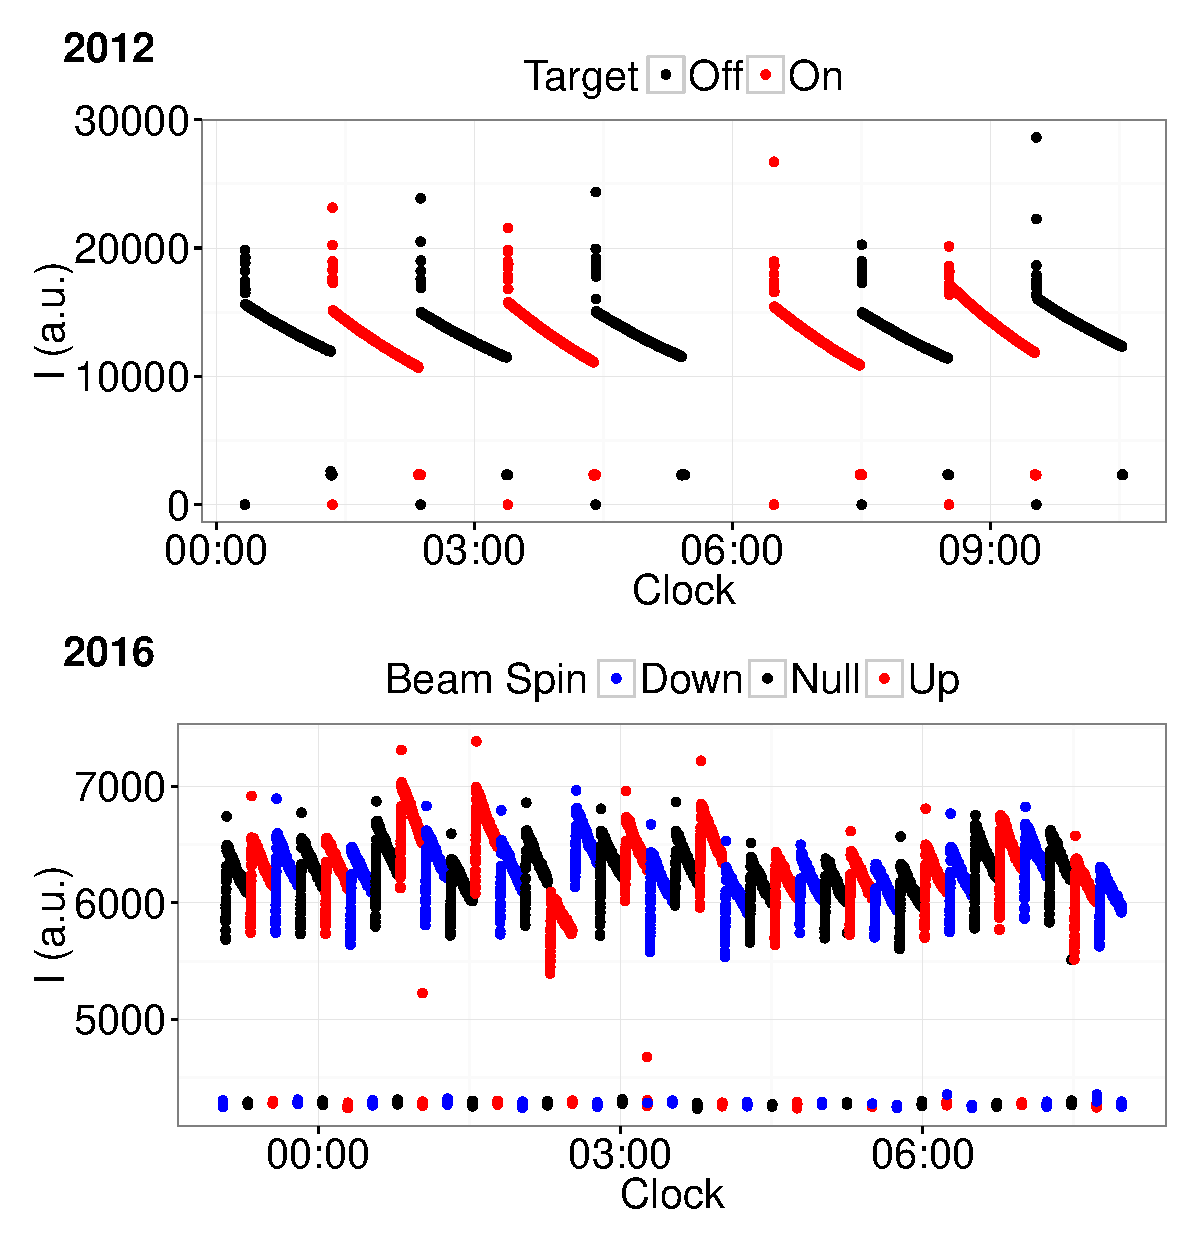
\includegraphics[scale=.8]{img/Cycles_12--16.eps}
		\caption{Средний ток пучка как функция времени. 
			Верхняя панель: эксперимент 2012 года. Циклы, измеренные со включённой мишенью окрашены красным, без мишени --- чёрным. Нулевые значения тока в начале каждого цикла вызваны значениями тока выше ёмкости данного АЦП.
			Нижняя панель: эксперимент 2016 года. Циклы окрашены в соответствии с направлением поляризации пучка (красный для направления спин вверх, синий для спин вниз, и чёрный для неполяризованного состояния. В первой половине цикла мишень была включена, во второй выключена.\label{fig:Cycles})}
	\end{figure}
	
	Статистические свойства циклов 2016 года собраны в Таблице~\ref{tbl:CycleChars}.
	
	\begin{center}
		\begin{table}
			\centering
			\begin{threeparttable}
				\caption{Характеристики типичного цикла 2016 года.\label{tbl:CycleChars}}
				\begin{tabular}{llr}
					\hline\hline
					Характеристика      & Тест             & P-величина \\ \hline
					Линейность          & Harvey-Collier   &        0\% \\
					-                   & Rainbow          &        0\% \\
					Постоянство наклона & Chow\tnote{a}    &      100\% \\
					-                   & Moving estimates &        1\% \\
					Гомоскедастичность  & Breusch-Pagan    &        0\% \\
					Автокорреляция      & Durbin-Watson    &        0\% \\ \hline\hline
				\end{tabular}
				\begin{tablenotes}
					\item[a]{Тест Chow был выполнен в каждой точке региона фитирования. Тестовой статистикой выбрано среднее значение F-статистик тестов.}
				\end{tablenotes}
			\end{threeparttable}
		\end{table}
	\end{center}

	\begin{figure}
		\centering
		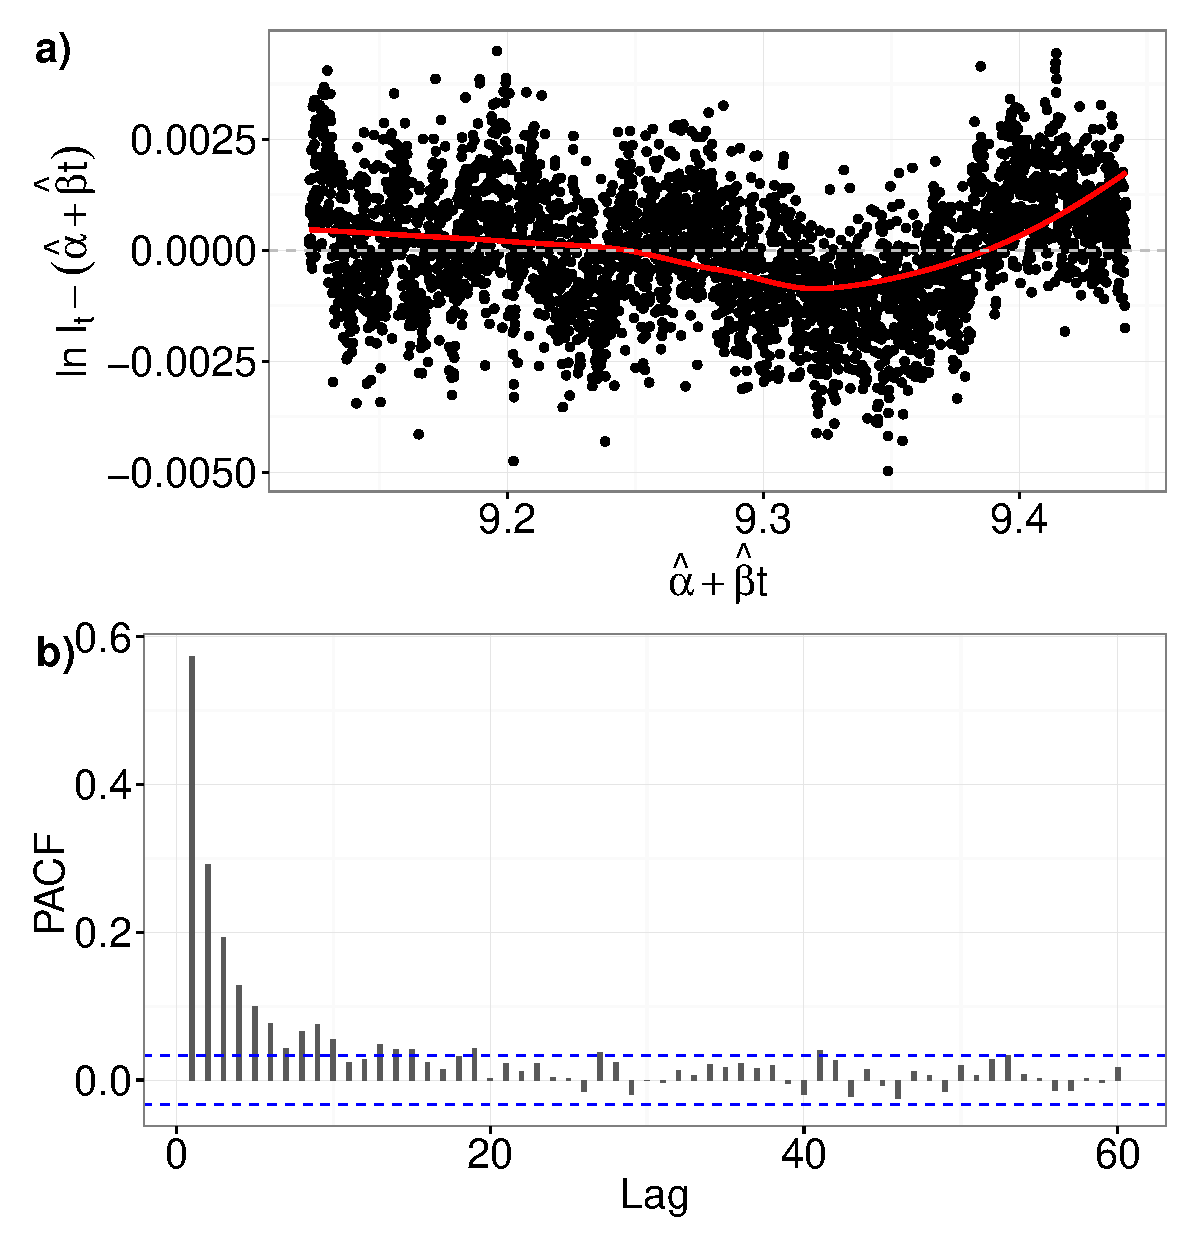
\includegraphics[scale=.8]{img/DiagPlot_969.eps}
		\caption{Диагностические зависимости типичного цикла 2016 года. a) Зависимость отклонений модели от фитированных значений. Изгиб красной линии свидетельствует о том, чтолинейная модель систематически недооценивает ток пучка в начале и конце цикла,  и переоценивает в середине. b) График функции частичной автокорреляции модельных отклонений; 95\% доверительный интервал отмечен прерванными горизонтальными линиями.\label{fig:Run969}}
	\end{figure}

	\subsection{Скорость рассеяния}
	Результаты фитирования циклов представлены в Таблице~\ref{tbl:Slp-big}. Результаты противоречат нашим ожиданиям, поскольку для циклов с включённой мишенью эффективное сечение должно увеличиваться для поляризации вверх, и уменьшаться для поляризации вниз, т.е. $\slp^+ < \slp^0 < \slp^-$; оценки, однако, удовлетворяют $\slp*^0 < \slp*^- < \slp*^+$. Это может свидетельствовать о неправильной маркировке спиновых состояний пучка. 
	
	Мы проверили эту гипотезу c помощью распределения $p(a,b) = \frac{\avg{a}-\avg{b}}{\sqrt{\SE{a}^2+\SE{b}^2}}$, и тестируя отличие разницы между средними значениями распределений наклона касательной между разными поляризационными группами от нуля. Средние значения статистически не различимы (P-величины T-тестов Вверх-Вниз, Вверх-Ноль, и Ноль-Вниз равны, соответственно: 72\%, 73\%, и 47\%); по этой причине, мы не имеем причин полагать что маркировка была неверна.
	
	\begin{center}
			\begin{threeparttable}[h]
			\centering
			\caption{Статистика фитирования циклов. \label{tbl:Slp-big}}
			\begin{tabular}{c|llrllrr}
				\hline\hline
				         Год          & Мишень               & Спин & \#\tnote{a} & Среднее [a.u.]   & Ошибка [a.u.] &  \\ \hline
				\multirow{2}{*}{2012} & Off                  & Null &           5 & $\vp{-9.04}{-5}$ & $\vp{6}{-7}$  &  \\
				                      & On                   & Null &           4 & $\vp{-1.20}{-4}$ & $\vp{1}{-6}$  &  \\ \hline
				\multirow{6}{*}{2016} & \multirow{3}{*}{Off} & Up   &          12 & $\vp{-2.26}{-4}$ & $\vp{7}{-6}$  &  \\
				                      &                      & Down &          12 & $\vp{-2.16}{-4}$ & $\vp{8}{-6}$  &  \\
				                      &                      & Null &          12 & $\vp{-2.12}{-4}$ & $\vp{9}{-6}$  &  \\
				                      & \multirow{3}{*}{On}  & Up   &          12 & $\vp{-2.51}{-4}$ & $\vp{4}{-6}$  &  \\
				                      &                      & Down &          12 & $\vp{-2.53}{-4}$ & $\vp{5}{-6}$  &  \\
				                      &                      & Null &          12 & $\vp{-2.54}{-4}$ & $\vp{6}{-6}$  &  \\ \hline\hline
			\end{tabular}
			\begin{tablenotes}
				\item[a]{Размер сэмпла.}
			\end{tablenotes}
		\end{threeparttable}
	\end{center}
	
	\subsection{Эффективное сечение}
	
	При определении эффективного сечения были использованы только соседние циклы. Так было сделано для того, чтобы минимизировать влияние дрифта переменных среды (таких как толщина мишени, которая была оценена дрифтовать на $0.5~ \sfrac{\%}{\mathrm{h}}$). Толщина мишени, использованная в оценках, была получена путём измерения спектра Шоттки,~\cite{Stein} которое было сделано один раз за весь эксперимент. Результаты оценки представлены в Таблице~\ref{tbl:CS-all}. Оценки, основанные на слопах, не прошедших тест Таки, маркированы как Unsound. Для сравнения, также представлены оценки, основанные на удалённых друг от друга циклах (обозначенные как Far).
	
	\begin{table}
		\centering
		\begin{threeparttable}
			\caption{Статистика эффективного сечения рассеяния. \label{tbl:CS-all}}
			\begin{tabular}{c|llrcr}
				\hline\hline
				         Год          & Звучность & Близость &  \# & Среднее\tnote{a} [a.u.] & Ошибка [a.u.] \\ \hline
				\multirow{4}{*}{2012} & Sound     & Close    &   4 &        507(507)         &             7 \\
				                      & Sound     & Far      &   8 &        553(563)         &            14 \\
				                      & Unsound   & Close    &   3 &        562(580)         &            36 \\
				                      & Unsound   & Far      &   5 &        515(512)         &            20 \\
				                      & All       &          &  20 &        536(544)         &            10 \\ \hline
				\multirow{4}{*}{2016} & Sound     & Close    &  40 &        409(411)         &            48 \\
				                      & Sound     & Far      &  92 &        396(385)         &            34 \\
				                      & Unsound   & Close    &   4 &       1400(1418)        &           170 \\
				                      & Unsound   & Far      &   8 &       1453(1457)        &            69 \\
				                      & All       &          & 144 &        486(473)         &            35 \\ \hline\hline
			\end{tabular}
			\begin{tablenotes}
				\item[a] Значение в скобках --- вариационное средне-взвешенное.
			\end{tablenotes}
		\end{threeparttable}
	\end{table}	

	\subsection{Асимметрия}\label{sec:Asymmetry}	
	Асимметрия была вычислена в соответствии с уравнением~\eqref{eq:AyyEst}. В этом выражении, мы использовали толщину мишени, вычисленную по спектру Шоттки~\cite{Stein} ($1.1\cdot 10^{14}$ cm$^{-2}$), и нашу лучшую оценку неполяризованного сечения (411 mb, см Tаблицу~\ref{tbl:CS-all}).
	
	\begin{figure}[h]
		\centering
		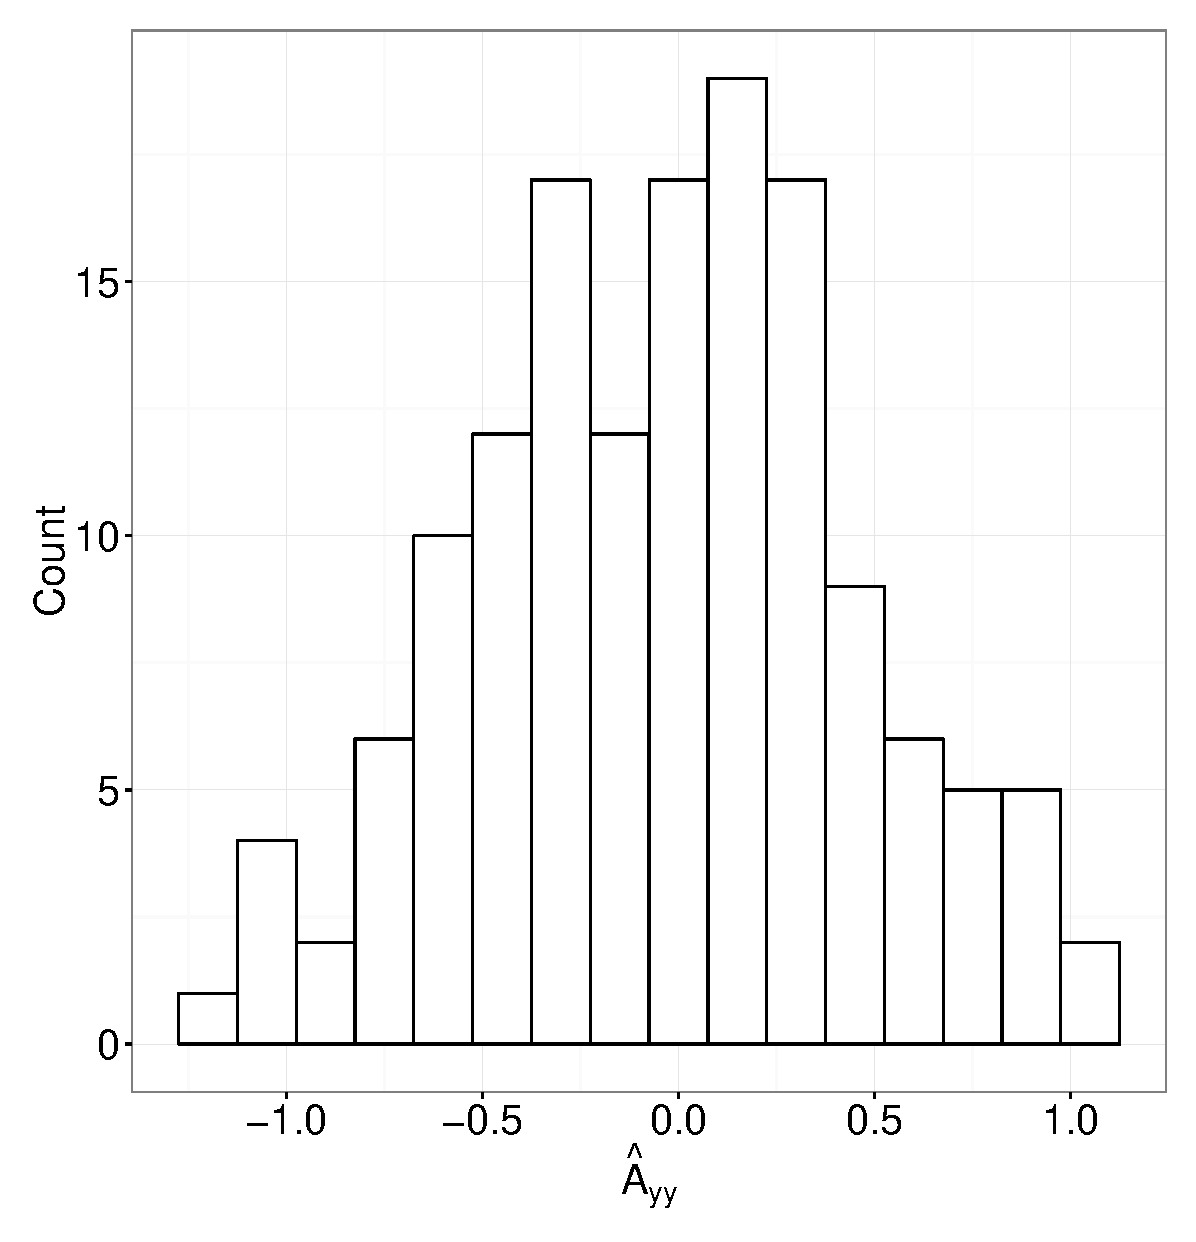
\includegraphics[scale=.8]{img/Ayy_dens.eps}
		\caption{Распределение асимметрии $\Ayy*$ полного сечения дважды-поляризованного рассеяния в протон-дейтрон рассеянии.\label{fig:AyyDensity}}
	\end{figure}
	
	\section{Анализ систематических ошибок}
	На Рис.~\ref{fig:Slopes} представлена зависимость оценки скорости рассеяния от времени для циклов с различной поляризацией пучка. Мы можем наблюдать статистически значимое увеличение времени жизни пучка с поляризацией вверх, уменьшение времени жизни пучка с поляризацией вниз, и статистически незначительный рост времени жизни неполяризованного пучка в циклах без мишени. Такая структура зависимости может свидетельствовать о том, что поляризация инжектированного пучка спадала со временем. 
	
	\begin{figure}[h]
		\centering
		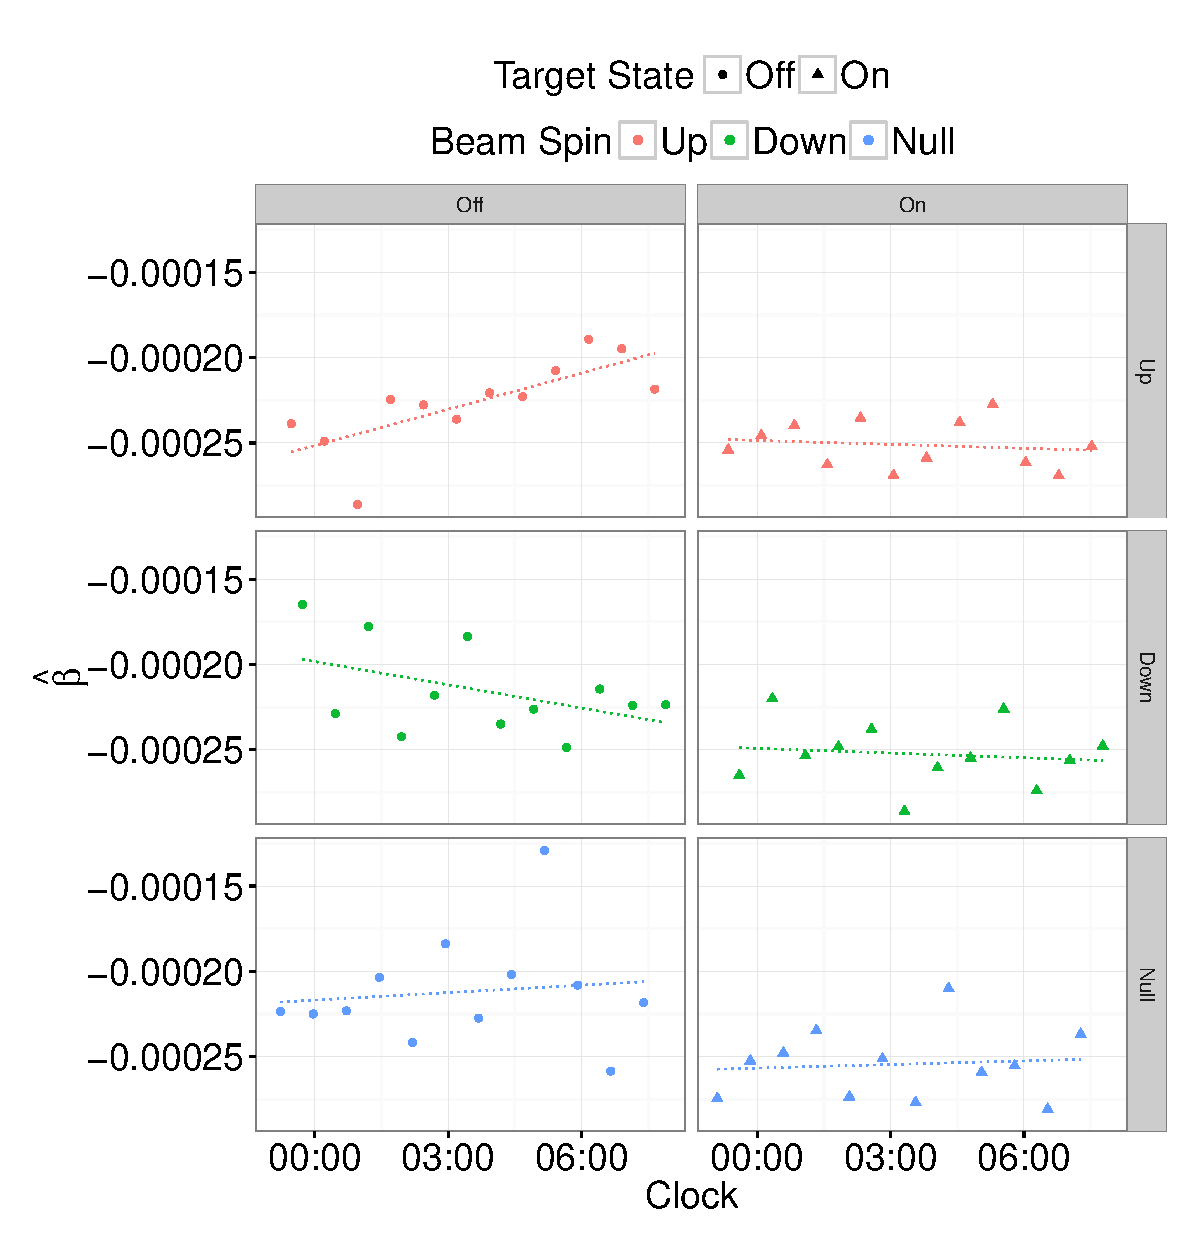
\includegraphics[scale=.8]{img/Slopes2016_VS_Clock.eps}
		\caption{Оценки угла наклона касательной в зависимости от времени, разделённые в соответствии с поляризацией пучка и присутствием мишени.\label{fig:Slopes}}
	\end{figure}
	
	Распределения коэффициента автокорреляции модельных отклонений представлены на Рис.~\ref{fig:DW2}. Положительная автокорреляция свидетельствует об инертности системы, увеличивает неопределённость оценки наклона касательной, но не влияет на её консистентность, если только она не вызвана наличием скрытого предиктора. 

	\begin{figure}[h]
		\centering
		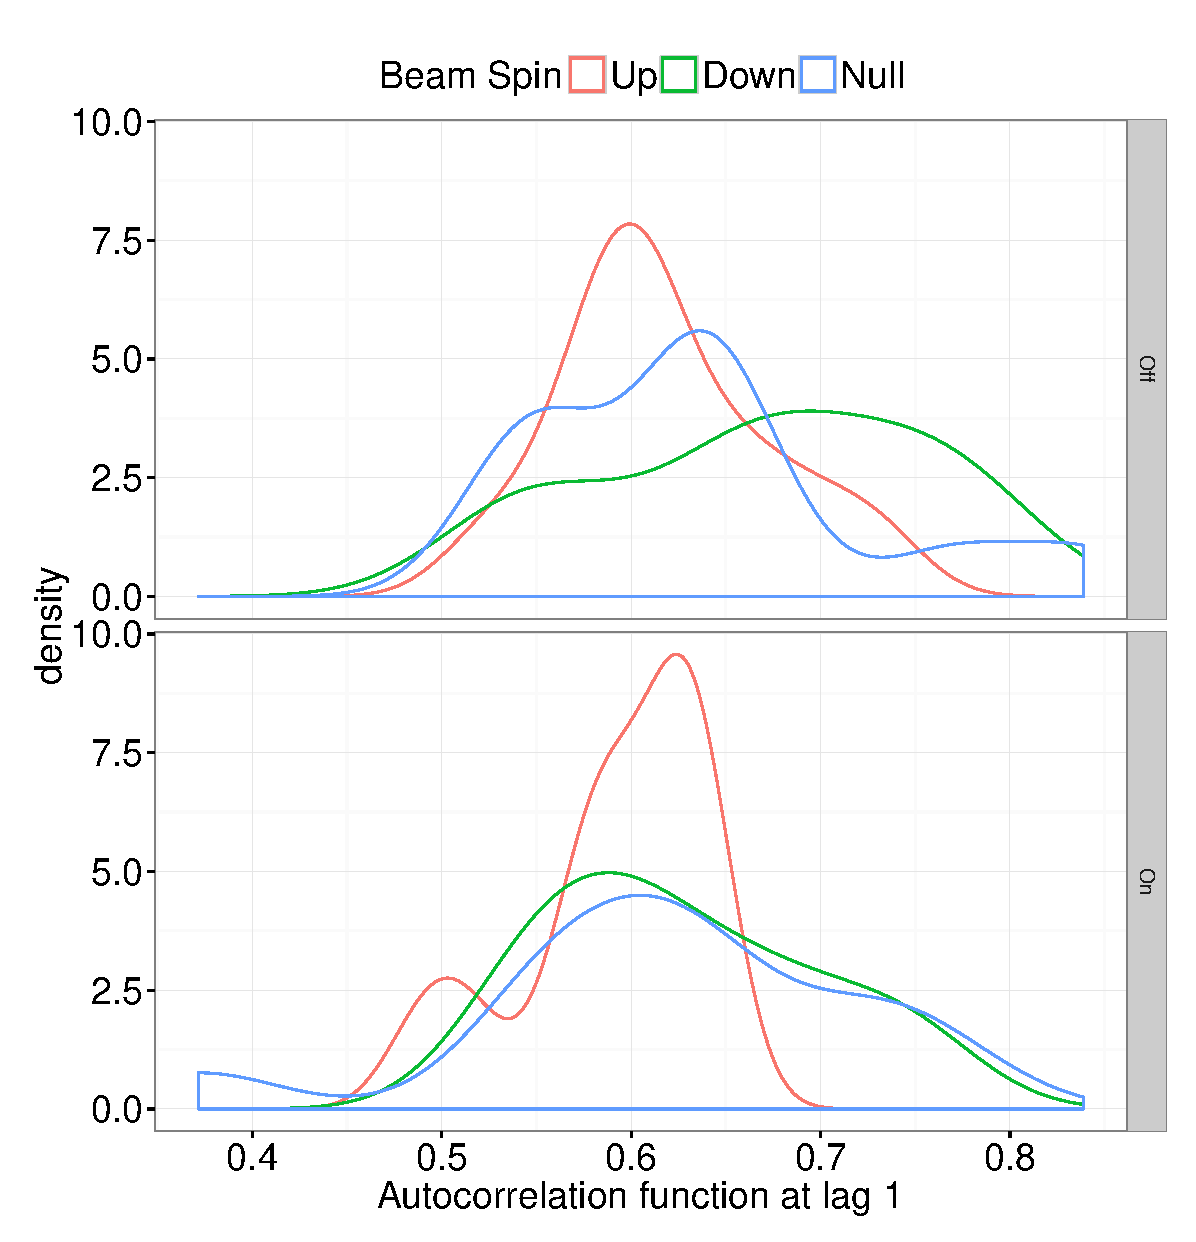
\includegraphics[scale=.8]{img/ACF1_dens.eps}
		\caption{Распределение автокорреляции первого порядка модельного отклонения.\label{fig:DW2}}
	\end{figure}

	Распределения точек структурных изменений в данных представлены на Рис.~\ref{fig:FStat_BP_dens}. На данный момент, рабочей гипотезой, объясняющей перелом в наклоне касательной, является изменение скорости откачки вакуума при низких давлениях.
	
	\begin{figure}[h]
		\centering
		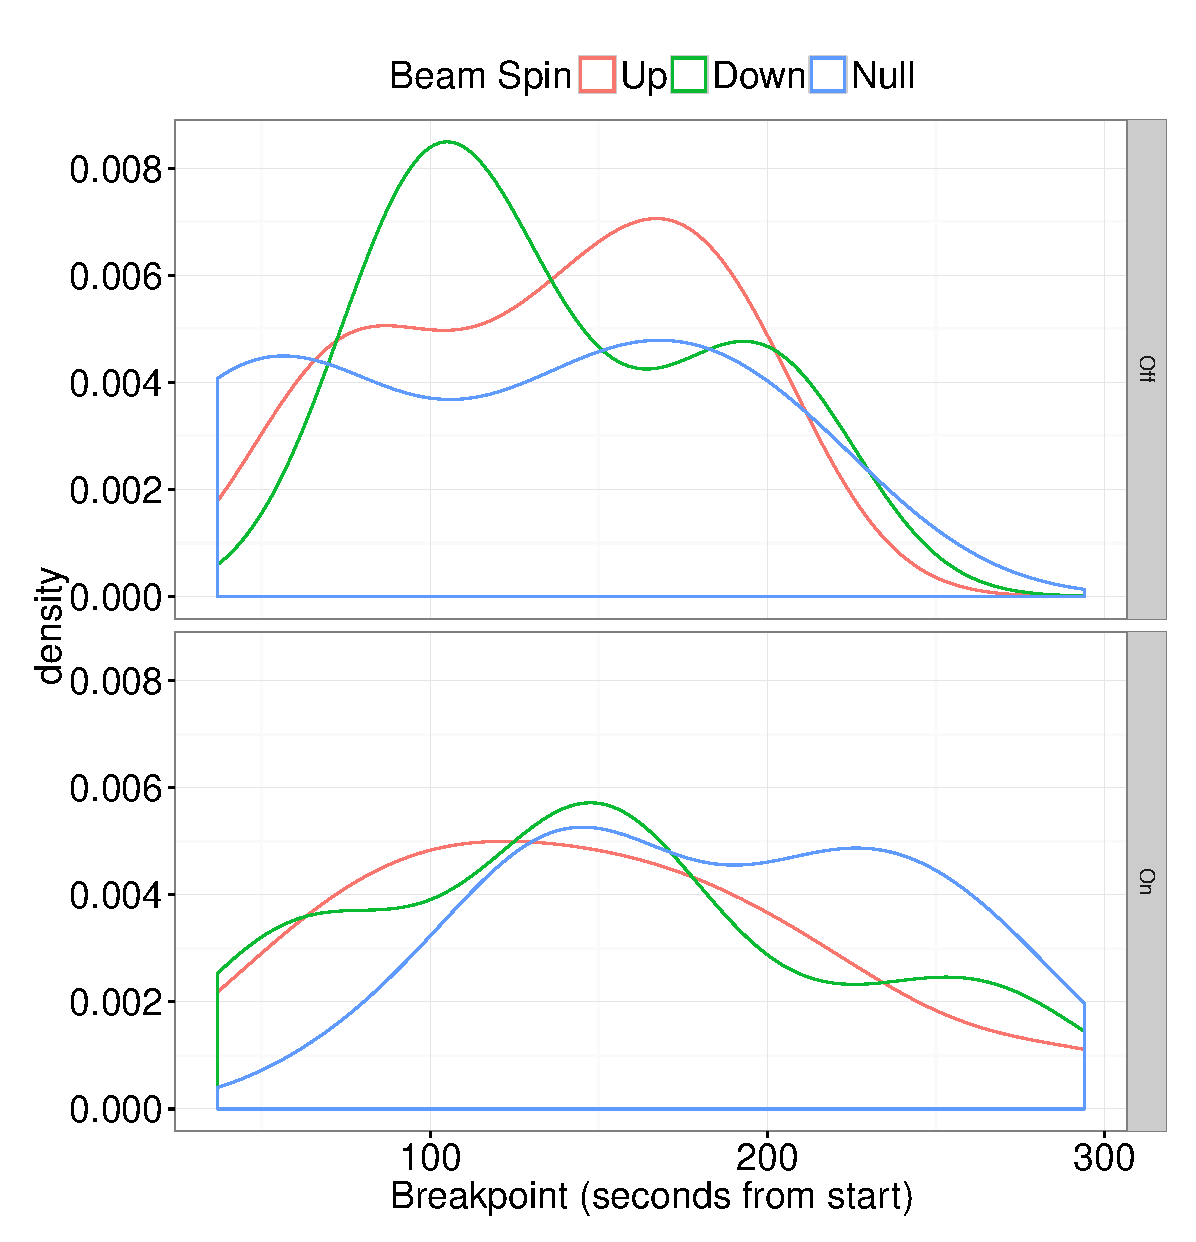
\includegraphics[scale=.8]{img/FStats_BP_dens.eps}
		\caption{Точка изменения величины наклона касательной, полученная движущимся тестом Чоу. Распределение циклов без мишени в верхней панели.\label{fig:FStat_BP_dens}}
	\end{figure}

	\section{Статистические требования к проведению эксперимента}\label{sec:StatReq}
	\newcommand{\Dim}[1]{\mathrm{#1}}
	\newcommand{\Tint}{\Delta t}
	\newcommand{\err}{\epsilon}
	\newcommand{\DP}{\Delta P}
	\DeclareDocumentCommand{\v}{m}{\sigma^2\bkt*{#1}}
	
	В оценках ниже использовались значения Таблицы~\ref{tbl:Param}.

	\begin{table}[h]
		\centering
		\caption{Значения параметров (Июнь 2016)\label{tbl:Param}}
		\begin{threeparttable}[h]
			\begin{tabular}{p{4.5cm}llr}
				\hline\hline
				Параметр                                         & Символ            & Величина           &             Размерность \\ \hline
				Частота оборота пучка                            & $\nu$             & 0.79               &                     MHz \\
				Толщина мишени                                   & $\Thick$          & $1.1\cdot 10^{14}$ & $\Dim{at\cdot cm^{-2}}$ \\
				Поляризация мишени                               & $P^t$             & 0.88               &                      -- \\
				Разница пооляризаций пучка спин-вверх--спин-вниз & $\DP$             & 1.48               &                      -- \\
				сечение $pd$ рассеяния                           & $\CS[0]$\tnote{a} & 70                 &                      mb \\ \hline
			\end{tabular}
			\begin{tablenotes}
				\item[a]{Из Particle Data Group \url{http://pdg.lbl.gov/2016/hadronic-xsections/rpp2014-pd_pn_plots.pdf}}
			\end{tablenotes}
		\end{threeparttable}
	\end{table}
	
	Стандартная ошибка среднего значения распределения оценок асимметрии $\SE{\avg{\Ayy*}}$ выражается через полную длительность эксперимента $H$ как
	\begin{equation}\label{eq:AvgAyySEPhys}
	\SE{\avg{\Ayy*}} = 4\sqrt{3}C\cdot \frac{\sqrt{\Tint}}{h\sqrt{H}}\cdot\SE{\err}.
	\end{equation}
	
	В связи с собственной вариацией наклона касательной, существует оптимальный размер статистики, дающий статистическую ошибку сравнимую с систематической ошибкой. Из выражения
	\begin{equation}
		\v{\avg{\Ayy*}}	= \frac{4 C^2}{H}\bkt{12\Tint\cdot\frac{\v{\err}}{h^2} + h\cdot\v{\slp}}.
	\end{equation}
	мы получаем оптимальное время измерения
	\begin{equation}
	h_{best} = \sqrt[3]{24\cdot \Tint} \bkt{\frac{\v{\err}}{\v{\slp}}}^{1/3}.
	\end{equation}
	
	Значение наилучшей достижимой точности в оценке среднего и длительность цикла, соответствующая ей, в зависимости от разрешения измерений тока, представлены в Таблице~\ref{tbl:SEAyy_varb} и на Рис.~\ref{fig:SEAyy_varb}. 
		
	Поскольку наклон касательной по определению
	\[
	\slp[t] = \frac{\Delta \ln I_t}{\Delta t} \approx \frac{1}{\Delta t}\frac{\Delta I_t}{I_t} \propto \frac{\Delta N_t}{N_t}, ~\Delta N_t \sim B(N_t, p),
	\]
	собственная вариабильность наклона касательной $\v{\slp}$ была оценена как стандартное отклонение вероятности рассеяния частицы 
	\begin{equation*}
	\begin{cases}
	\Xpct{\slp[t]} 	&= p, \\
	\SE{\slp[t]}		&= \frac{1}{\Delta t}\frac{\sqrt{p(1-p)}}{\sqrt{N_t}}, \\
	p 				&= \nu\CS[0]\Thick\Delta t.
	\end{cases}
	\end{equation*}
	
	Для значений из Таблицы~\ref{tbl:Param}, $\v{\slp} \approx 8\cdot 10^{-16}$.
	
	\begin{table}[h]
		\centering
		\caption{Наилучшая достижимая точность $\SE{\avg{\Ayy*}}$.\label{tbl:SEAyy_varb}}
		\begin{tabular}{lrr}
			\hline\hline
			$\SE{\err}$			&	$h_{best}$ (min)	& $\SE{\avg{\Ayy*}}$\\
			\hline
			$5\cdot10^{-3}$		&	141					& $8\cdot10^{-4}$\\
			$1\cdot10^{-3}$		&	48					& $3\cdot10^{-4}$\\
			$5\cdot10^{-4}$		&	30					& $3\cdot10^{-4}$\\
			$1\cdot10^{-4}$		&	10					& $2\cdot10^{-4}$\\
			$5\cdot10^{-5}$		&	7					& $1\cdot10^{-4}$\\
			\hline
		\end{tabular}
	\end{table}

	\begin{figure}[h]
		\centering
		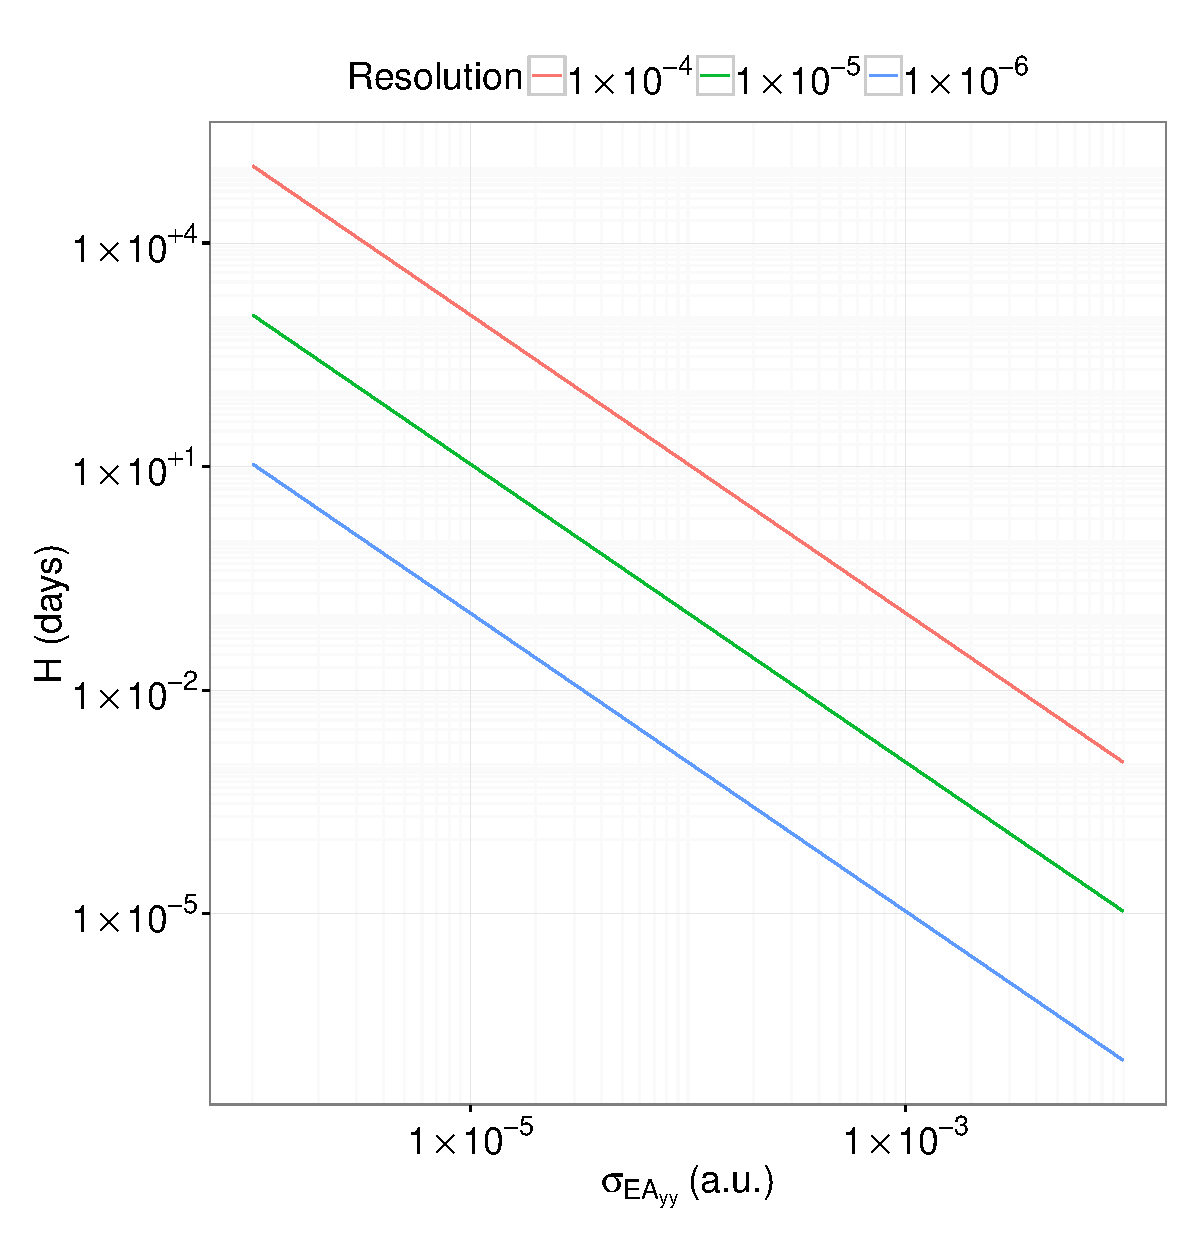
\includegraphics[scale=.8]{img/BeamTime_15minCycles.eps}
		\caption{Необходимое время эксперимента (в полных днях) как функция стандартной ошибки среднего оценки $\Ayy$, в случае 15-минутных циклов.\label{fig:BeamTime}}
	\end{figure}
	\begin{figure}[h]
		\centering
		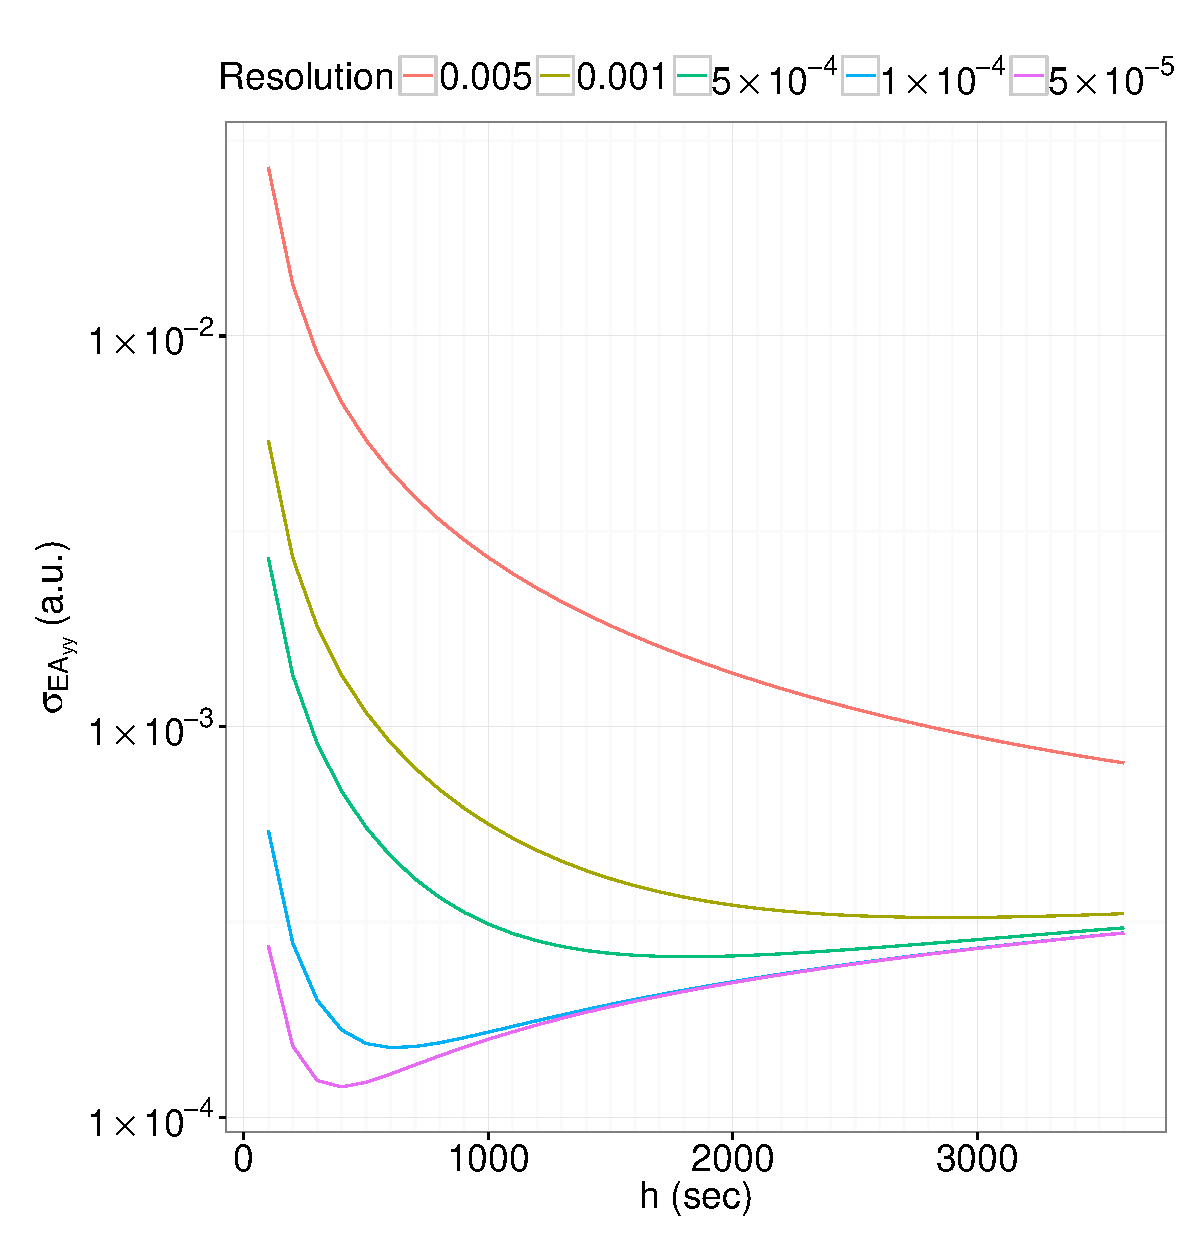
\includegraphics[scale=.8]{img/SEAyy_varB_15min.eps}
		\caption{Стандартная ошибка средней оценки $\Ayy$ как функция длительности цикла при собственной вариации скорости рассеяния $\v{\slp} = 1\cdot10^{-15}$.\label{fig:SEAyy_varb}}
	\end{figure}
	
	\pagebreak
	\begin{thebibliography}{99}
		
		\bibitem{Sakharov}
		D. V. Perepelitsa
		\textsc{Sakharov Conditions for Baryogenesis}.
		Columbia University Department of Physics,
		2008.
		
		\bibitem{Conzett}
		H.E. Conzett,
		7th Int. Conf. on "Pol. Phen. Nucl. Phys.," Paris (1990) 2D.
		
		\bibitem{Proposal}
		R. Beck, P.D. Eversheim, F. Hinterberger et al.,
		Cosy Proposal \# 215:
		\textsc{Test of Time-Reversal Invariance in Proton-Deuteron Scattering at 
			COSY}.
		Helmholtz Institut für Strahlen- und Kernphysik, University Bonn, Germany.
		
		\bibitem{Weidemann}
		C. Weidemann, F. Rathmann, et al. Phys. Rev. ST Accel. Beams \textbf{18}, 2 (2015).
		
		\bibitem{Stein}
		H. J. Stein, M. Hartmann, I. Keshelashvili, et al., Phys. Rev. ST Accel. Beams \textbf{11}, 052801 (2008).
		
		\bibitem{Sinervo}
		Pekka K. Sinervo
		\textsc{Definition and Treatment of Systematic Uncertainties in High Energy Physics and Astrophysics}.
		PHYSTAT2003, SLAC, Stanford, California, 
		September 8-11, 2003.
		
		\bibitem{SeasonalErrors}
		Christian Servin, Martine Ceberio, Aline James, et al.
		\textsc{How to Describe and Propagate Uncertainty When Processing Time Series: Methodological and Computational Challenges, with Potential Applications to Environmental Studies}.
		Cyber-ShARE Center, University of Texas at El Paso, El Paso, TX 79968, USA. 
		
		\bibitem{Symmetries}
		Marco S. Sozzi,
		\textsc{Discrete Symmetries and CP violation}.
		University of Pisa,
		2008.
		
		\bibitem{Lee&Yang}
		T. D. Lee, C. N. Yang,
		\textsc{Question of Parity Conservation in Weak Interactions}.
		Phys. Rev. 104 (1956) 254--258.
		
		\bibitem{Wu}
		C. S. Wu, E. Ambler et al.,
		\textsc{Experimental Test of Parity Conservation in Beta Decay}.
		Phys. Rev. 105 (1957) 1423--1415.
		
		\bibitem{Eversheim}
		P. D. Eversheim et al.,
		\textsc{Parity violation in proton proton scattering at 13.6 MeV}.
		Phys. Lett. B 256 (1991) 11-14.
		
		\bibitem{WASA-at-COSY_Hepi}
		P. Adlarson, W Augustyniak, W. Bardan et al.,
		\textsc{Charge Symmetry Breaking in $dd \to {}^4He \pi^0$ with WASA-at-COSY}.
		Phys. Lett. B 739 (2014) 44–49.
		
		\bibitem{WASA-at-COSY-Henpi}
		P. Adlarson, W Augustyniak, W. Bardan et al.,
		\textsc{Investigation of the $dd \to {}^3He n \pi^0$ reaction with the FZ J\"{u}lich WASA-at-COSY facility}.
		Phys. Rev. C 88 (2013) 014004.
		
		\bibitem{CPLEAR}
		A. Angelopoulos et al.,
		\textsc{Physics at CPLEAR}. 
		Phys. Rep. 374 (2003) 165--270.
		
		\bibitem{BaBar}
		J. P. Lees, V. Poireau, V. Tisserand et al.,
		\textsc{Observation of Time-Reversal Violation in the $B^0$ Meson System}.
		Phys. Rev. Lett. 109 (2012) 211801.
		
		\bibitem{Goldstein}
		F. Arash, M.J. Moravcsik and G.R. Goldstein,
		Phys. Rev. Lett. 54 (1985) 2649.
		
		\bibitem{COSY}
		B. Lorentz, U. Bechstedt, J. Dietrich et al.,
		\textsc{Status of the cooler synchrotron COSY-Juelich}.
		Proc. of EPAC'04, Lucerne, Switzerland.
		
		\bibitem{JULIC}
		W. Br\"autingam, R. Brings, H. Jungwirth et al.,
		\textsc{H$^-$-operation of the cyclotron JULIC as injector for the cooler synchrotron COSY-J\"ulich}.
		Proc. of the 15th Intl. Conf. on Cyclotrons and their Applications, Caen, France.
		
		\bibitem{COSYaccNN}
		A. Lehrach, U. Bechstedt, J. Dietrich et al.,
		\textsc{ACCELERATION OF THE POLARIZED PROTON BEAM IN THE
			COOLER SYNCHROTRON COSY}.
		Proc. of PAC'99, New York City, 
		1999.
		
		\bibitem{PhDYe}
		Qiujian Ye,
		\textsc{Strangeness Production in Selected Proton-Induced
			Processes at COSY-ANKE}.
		Department of Physics in the Graduate School of Duke University,
		2013.
		
		\bibitem{Ohlsen}
		Gerald G Ohlsen
		\textsc{polarization transfer and spin correlation experiments in nuclear physics}.
		Los Alamos Scientific Laboratory, University of California, Los Alamos, New Mexico 87544, 
		1972.
		
		\bibitem{Barschel}
		Colin Barschel
		\textsc{calibration of the Breit-Rabi polarimeter for the PAX spin-filtering experiment at COSY/J\"ulich and AD/CERN}.
		Faculty of Mathematics, Computer Science and Natural Sciences of RWTH Aachen,
		2010.
		
		
		%%%%%%%%%%%%%%%%%%%%%%%%%%%%%%%%%%%%%%%%%%%%%%%%%%%%%%%%%%%%%%%%%%%%%%%%%%%%%%%%5
		
		\bibitem{tensors}
		Kees Dullemond \& Kasper Peeters
		\textsc{Introduction to Tensor Calculus}.
		University of Nijmegen / University of Amsterdam.
		
		
		\bibitem{Barlow}
		Roger Barlow
		\textsc{Systematic Errors: Facts and Fictions}.
		Department of Physics, Manchester University, England,
		2002.
		
		\bibitem{Samuel}
		Deepak Samuel
		\textsc{Test of Feasibility of a Novel High Precision Test of Time Reversal Invariance}.
		Mathematisch-Naturwissenschaftlichen Fakult\"{a}t der Rheinischen Friedrich-Wilhelms-Universit\"{a}t Bonn,
		2007.
		
		\bibitem{Gaisser}
		Martin Gai\ss er
		\textsc{Simulations of the Atomic Beam Transport in an Atomic Beam Source under the influence of Spin-Selective Sextupole Magnets}.
		Mathematisch-Naturwissenschaftlichen Fakult\"{a}t der Universit\"{a}t zu K\"oln,
		2013.
		
		%%%%%%%%%%%%%%%%%%%%%%%%%%%%%%%%%%%%%%%%%%%%%%%%%%%%%%%%%%%%%%%%%%%%%%%%%%%%%%%%%%%	
		
	\end{thebibliography}
	
\end{document}